% This file was converted to LaTeX by Writer2LaTeX ver. 1.4
% see http://writer2latex.sourceforge.net for more info
\documentclass[a4paper]{article}
\usepackage[utf8]{inputenc}
\usepackage[T1]{fontenc}
\usepackage[ngerman]{babel}
\usepackage{amsmath}
\usepackage{amssymb,amsfonts,textcomp}
\usepackage{color}
\usepackage{array}
\usepackage{hhline}
\usepackage{hyperref}
\hypersetup{pdftex, colorlinks=true, linkcolor=blue, citecolor=blue, filecolor=blue, urlcolor=blue, pdftitle=}
\usepackage[pdftex]{graphicx}
% footnotes configuration
\makeatletter
\renewcommand\thefootnote{\arabic{footnote}}
\makeatother
% Outline numbering
\setcounter{secnumdepth}{0}
% Page layout (geometry)
\setlength\voffset{-1in}
\setlength\hoffset{-1in}
\setlength\topmargin{2cm}
\setlength\oddsidemargin{3.5cm}
\setlength\textheight{22.706001cm}
\setlength\textwidth{15.500999cm}
\setlength\footskip{1.497cm}
\setlength\headheight{0.998cm}
\setlength\headsep{0.499cm}
% Footnote rule
\setlength{\skip\footins}{0.119cm}
\renewcommand\footnoterule{\vspace*{-0.018cm}\setlength\leftskip{0pt}\setlength\rightskip{0pt plus 1fil}\noindent\textcolor{black}{\rule{0.25\columnwidth}{0.018cm}}\vspace*{0.101cm}}
% Pages styles
\makeatletter
\newcommand\ps@Standard{
  \renewcommand\@oddhead{\sffamily INM - Potentielle Neuordnung des Informationsmanagements\hfill 02.06.15}
  \renewcommand\@evenhead{\@oddhead}
  \renewcommand\@oddfoot{\sffamily INM – SoSe 2015\hfill \hfill \thepage{} / ?}
  \renewcommand\@evenfoot{\@oddfoot}
  \renewcommand\thepage{\arabic{page}}
}
\makeatother
\pagestyle{Standard}
\title{}
\begin{document}
\section[1.3.5\ \ Qualitätsmanagement der Informationsprozesse]{1.3.5\ \ Qualitätsmanagement der Informationsprozesse}
{\sffamily
Im Folgenden wird der Qualitätsmanagement-Prozess in seinen Grundzügen definiert, am konkreten Beispiel der Minimierung
von Durchlaufzeiten genauer betrachtet und praktisch mit Hilfe der IT Balanced Scorecard durchexerziert. Abschließend
wird erörtert, welche Besonderheiten hierbei an Hochschulen bestehen und Möglichkeiten aufgezeigt, diese
Schwierigkeiten zu umgehen. }

\subsection[1.3.5.1 \ \ Aufgaben des Qualitätsmanagements ]{1.3.5.1 \ \ Aufgaben des Qualitätsmanagements }
{\sffamily
In einem Informationsmanagement bildet das Qualitätsmanagement der Informationsprozesse einen zentralen Aufgabenbereich.
Es übernimmt die Planung, Koordination und Steuerung der Informationsflüsse und prüft fortwährend, inwieweit eine
Nutzbarkeit und Effizienz der Prozesse in der Realität gewährleistet ist, um deren Qualität gegebenenfalls mit
gezielten Maßnahmen zu optimieren. \footnote{Schröder, Späne, Schröder 2005, 34 ff.}}


\bigskip

{\sffamily
Hierzu fungiert ein Team von Qualitätsmanagern als Vermittler zwischen den verschiedenen Parteien im Unternehmen und
überbrückt potentiell auftretende Kommunikations- oder Kulturbarrieren, um eine zielorientierte und effiziente
Informationsversorgung der beteiligten Parteien zu ermöglichen. }


\bigskip

{\sffamily
Zu Beginn des Qualitätsmanagement-Prozesses gilt es, eine Leitstrategie aufzustellen. Hierfür wird der aktuelle
Ist-Zustand des Unternehmens in Bezug auf seine Organisation von Informationsflüssen analysiert. Dabei zum Vorschein
kommende Schwachstellen werden erfasst und durch mögliche optimierende Handlungsoptionen ergänzt. \footnote{Helmke,
Uebel 2013.}}


\bigskip

{\sffamily
Während der Durchführung der neu erschaffenen Maßnahmen ist das Qualitätsmanagement-Team mit der stetigen Überwachung
dieser betraut. Bereits bei kleinen Abweichungen vom Plan kann mit gegensteuernden Maßnahmen eingegriffen werden. Eine
im Voraus aufgestellte Zeitplanung ist hierbei ebenso wichtig wie eine klare Definition der Zuständigkeiten im
Qualitätsmanagement-Team, um eine termingerechte Erreichung der gesetzten Ziele noch zu garantieren.}


\bigskip

{\sffamily
Nach Ablauf des gesetzten Zeitrahmens oder nach Beendigung der Maßnahmen ist es erforderlich, mittels einer sogenannten
Feedback-Analyse festzustellen, inwieweit das gesteckte Ziel erreicht wurde und aus welchen Gründen es nicht zu 100\%
zufriedenstellenden Ergebnissen kommen konnte. Die hieraus resultierenden Erkenntnisse bilden daraufhin die Grundlage
für eine anschließende Feedforward-Analyse, die die weitergehend erforderlichen Maßnahmen feststeckt, um in einer
weiteren Phase die Zielerreichung durch verbesserte Maßnahmen zu garantieren. \footnote{Gadatsch 2012.}}

\subsection[1.3.5.2 \ \ Prozessoptimierung durch Minimierung der Durchlaufzeiten]{1.3.5.2 \ \ Prozessoptimierung durch
Minimierung der Durchlaufzeiten}
{\sffamily
Essenzielles Ziel des Qualitätsmanagement-Teams ist es, anhand bewährter Vorgehensweisen die Durchlaufzeiten von
Informationen zu minimieren. Hierdurch wird der Informationsfluss quantitativ und qualitativ verbessert, da bestehende
Abhängigkeiten der Parteien in Bezug auf die Informationen schneller bedient werden können und somit durch minimierte
Wartezeiten eine beträchtliche Budgetersparnis resultiert. }


\bigskip


\bigskip


\bigskip

{\sffamily
Wie in Abbildung 1 erkennbar, existieren elementare Methoden zur Reduktion von Durchlaufzeiten nach Bleicher aus dem
Jahre 1991, die noch heute ihre Gültigkeit in der Anwendung haben. }

\begin{figure}
\centering
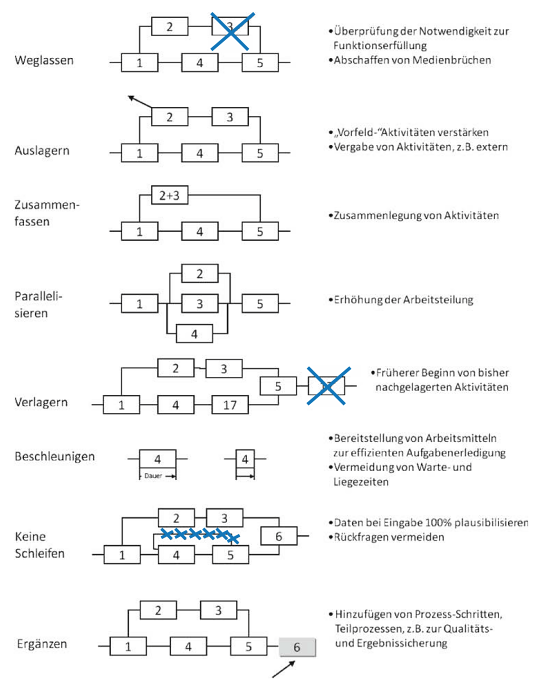
\includegraphics[width=15.5cm,height=20.511cm]{miriamkapitel135136-img/miriamkapitel135136-img001.png}
\caption[Minimierung von Durchlaufzeiten nach Bleicher 1991, 196.]{Minimierung von Durchlaufzeiten nach Bleicher 1991,
196.}

\end{figure}

\bigskip

{\sffamily
Insbesondere das Zusammenfassen von Aktivitäten hat den entscheidenden Vorteil, dass Abstimmungsprozesse und
Abhängigkeiten zwischen mehreren Parteien entfallen und somit die Umsetzungsdauer auf ein Minimum reduziert wird. }


\bigskip

{\sffamily
Auch die Methode des Parallelisierens sollte in den Fokus gerückt werden. Wie in Abbildung 1 ersichtlich, werden hierbei
mehrere Parteien, die für eine darauffolgende Partei relevant sind, zeitgleich geschaltet, um Wartezeiten zu
verhindern. }


\bigskip

{\sffamily
Zu guter Letzt sei das Ergänzen von Prozessschritten betont. Auf den ersten Blick scheint diese Methode paradox, da
durch Ergänzung weiterer Parteien der Zeit- und Arbeitsaufwand vorerst erhöht wird. Durch einen globaleren Blick wird
schnell deutlich, dass ohne diese Parteien zu einem späteren Zeitpunkt Problematiken entstehen können, die in ihrer
Lösung viel zeit- und arbeitsintensiver sind und das Unternehmen in seiner Prozessqualität deutlich zurückwerfen
könnte.}


\bigskip

{\sffamily
Die in Abbildung 1 gezeigten Methoden zur Durchlaufzeit-Minimierung sollten also vom Qualitätsmanagement-Team von Beginn
an in die Planung mit einbezogen werden, da mit minimalem Aufwand eine weitreichende, inhaltlich und finanziell
positive Auswirkung auf die Qualität des Gesamtprozesses erzeugt wird. }

\subsection[1.3.5.3 \ \ Anwendung des Qualitätsmanagements am Beispiel der IT Balanced Scorecard]{1.3.5.3 \ \ Anwendung
des Qualitätsmanagements am Beispiel der IT Balanced Scorecard}
{\sffamily
Das strategisch-operative Konzept für eine qualitative Unternehmenssteuerung aus den 90er Jahren von R. S. Kaplan und D.
P. Norton hat sich im Laufe der Zeit zum Standardinstrument entwickelt. \footnote{Friedag, Schmidt 2004.} Grundlegend
für die IT Balanced Scorecard ist das Schema Eingabe → Verarbeitung → Ausgabe → Resultat. Die Kombination von Qualität
der Mitarbeiter, Kundenorientierung und finanzielle Ziele ermöglicht die Generierung und Sicherung eines gelungenen
Informationsmanagements. \footnote{Gabriel, Beier 2003.} }


\bigskip


\bigskip

{\sffamily
Die IT Balanced Scorecard zeichnet sich – wie in Abbildung 2 deutlich wird – durch eine stetige Feedback- und
Feedforward-Kommunikation aus. Zu Beginn des Managementprozesses werden in der Phase „Planung und Vorgaben“ die
grundlegenden Ziele des Unternehmens definiert. In einem nächsten Schritt werden in der Phase „Vision und Strategie“
Kernaussagen zur Strategiefindung erarbeitet, insbesondere im Hinblick auf den Zusammenhang von Ursache und Wirkung,
und Optimierungsmöglichkeiten zusammengestellt. Das Handlungskonzept wird in „Feedback und Lernen“ final ausformuliert
und in der vierten Phase „Kommunikation und Verbindung“ mit der Strategie und übergeordneten Zielen verknüpft. Eine
detaillierte Dokumentation von Teilzielen erhöht in dieser Phase die Motivation der Mitarbeiter zur Zielerreichung.
\footnote{Kaufmann 2002, 35 ff.} }

\begin{figure}
\centering
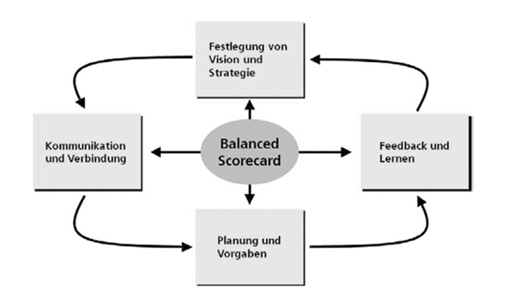
\includegraphics[width=15.502cm,height=10.145cm]{miriamkapitel135136-img/miriamkapitel135136-img002.jpg}
\caption[IT Balanced Scorecard Kreislauf nach Gadatsch 2012.]{IT Balanced Scorecard Kreislauf nach Gadatsch 2012.}

\end{figure}
{\sffamily
Die Definition von klaren Zielen, Bedingungen und Kennzahlen generiert ein komplexes Kennzahlensystem, welches durch
Herunterbrechen der Strategie auf operatives Handeln einen ganzheitlichen Überblick über die interne Organisation des
Unternehmens liefert. Die Einbeziehung von Ursache und Wirkung vereinfacht die vorausschauende Unternehmensführung und
ergänzt die Sichtweise auf das Unternehmen zu einem ausgewogenen (balanced) Bild. }


\bigskip

{\sffamily
Da die Möglichekeiten zur Befüllung der Scorecard sehr vielseitig sind, sollte vermieden werden, sie mit zu vielen
komplexen Zahlen zu überladen. Im Fokus stehen bei diesem Konzept vorrangig die Maßnahmenfindung unter Berücksichtigung
von Ursache und Wirkung, was durch eine einseitige Betrachtung der Kennzahlen zu sehr in den Hintergrund rücken und den
Lösungsprozess negativ belasten könnte.}

\subsection[1.3.5.4 \ \ Besonderheiten an Hochschulen]{1.3.5.4 \ \ Besonderheiten an Hochschulen}
{\sffamily
Ein gut funktionierendes Qualitätsmanagement kann nur effektiv und reibungslos funktionieren, wenn es an zentraler
Stelle nahe des Entscheidungsträgers positioniert und gelebt wird. Die Umsetzungsverantwortung eines ganzheitlichen
Qualitätsmanagements liegt bei Hochschulen in der Regel bei der Hochschulleitung, die ihre Aufgaben im Prozess der
Informationsflussoptimierung begreifen und verantworten muss. }


\bigskip

{\sffamily
Eine der grundlegendsten Besonderheiten an Hochschulen liegt in der internen Strukturierung von Verantwortlichkeiten.
Die Hochschule ist unterteilt in Fachbereiche, welche geschlossen für sich arbeiten können, aber dennoch der
Hochschulleitung unterstellt sind. Zusätzlich zu diesen beiden Bereichen ist noch das Präsidium zu nennen, welches
insgesamt für eine effiziente Aufgabenerfüllung und Interessensvertretung der Hochschule verantwortlich ist.
\footnote{Mintzberg 1992, 353 ff. } }


\bigskip

{\sffamily
Im Zuge der Einführung eines geordneten Qualitätsmanagements gilt es also, die Positionierung nahe der Hochschulleitung
mit einer anwendungsbezogenen Platzierung innerhalb jedes Fachbereiches unter Einbeziehung des Präsidiums zu
verknüpfen, um ganzheitliche Lösungen zur Realisierung eines Qualitätsmanagements zu finden und umsetzen zu können. Ein
Außenvorlassen des Fachbereichs, in dem die Lösungen schließlich umgesetzt werden, ist faktisch unmöglich. Durch die
Vielzahl an Entscheidungsträgern und Mitredern besteht an Hochschulen ein höherer Bedarf an Kommunkations- und
Abstimmungsleistungen zwischen diesen als in anderen Institutionen und Unternehmen. Es besteht zudem die Gefahr, dass
Zuständigkeiten der verschiedenen Rollen an der entsprechenden Hochschule nicht klar geregelt sind, was die
Funktionsweise des Entscheidungsprozesses zwar bestenfalls nicht beeinträchtigt, dessen Ablauf allerdings sehr
unsystematisch gestaltet und den Fluß des Prozesses ausbremst.}


\bigskip

{\sffamily
Neben der strukturellen Schwierigkeiten in der Aufstellung eines Qualitätsmanagements besteht eine weitere Besonderheit
in der inhaltlichen Vereinheitlichung der Anforderungen der einzelnen Parteien, die im schlechtesten Fall sehr
verschieden sind oder sich gar widersprechen, sodass diese für alle Bereiche zentral gültig ist. }


\bigskip

{\sffamily
Mithilfe renommierter Werkzeuge, wie z.B. der IT Balanced Scorecard, liegt es nun in der Hand des
Qualitätsmanagement-Teams, die erarbeiteten Prozessstrategien und Maßnamen transparent für jeden Bereich der Hochschule
einsehbar zu publizieren und alle betreffenden Personen über Änderungen zu informieren. Die Kontrolle in den
Fachbereichen, ob und inwieweit die Maßnahmen zur Prozessoptimierung beitragen, darf hierbei nicht vernachlässigt
werden.
\footnote{https://www.evalag.de/dedievl/projekt01/media/pdf/qm/audit/evalag\_eckpunkte\_qualitaetsmanagement.pdf}}

\section[1.3.6\ \ Anwendung des Informationsmanagements am Beispiel von Hochschulen]{1.3.6\ \ Anwendung des
Informationsmanagements am Beispiel von Hochschulen}
{\sffamily\color{black}
Mit der praktischen Anwendung der bisher erörterten Erkenntnisse zum Thema Informationsmanagement an Hochschulen befasst
sich das nachfolgende Kapitel. Hierbei wird insbesondere analysiert, inwieweit der Bereich des Immatrikulations- und
Prüfungsamtes als zentraler Knotenpunkt in der Informationsverteilung dienen kann und welche Auswirkungen sich für die
Bibliothek und die Organisation von Rechnerpools ergeben können.}

\subsection[1.3.6.1 \ \ Immatrikulations{}- und Prüfungsamt ]{\color{black} 1.3.6.1 \ \ Immatrikulations- und
Prüfungsamt }
{\sffamily\color{black}
In Hochschulen, bei denen ein Informationsmanagement Anwendung findet, bildet das Immatrikulations- und Prüfungsamt eine
Art interne Informationszentrale, welche weitere Bereiche mit notwendigen Informationen versorgt. Betrachet an einem
Beispiel bedeutet dies Folgendes: Bei Immatrikulation eines neuen Studierenden wird diesem vom Immatrikulationsamt eine
Matrikelnummer zugewiesen und seine Stammdaten ins HIS eingepflegt. Nun ist es Aufgabe des Immatrikulationsamtes, das
HIS zu einer Art Schnittstelle für alle wichtigen Hochschulbereiche, wie z.B. die Bibliothek, die Mensa oder auch die
Verwaltung von Computerräumen, zu machen, sodass diese Bereiche via Eingabe der Matrikelnummer auf für sie wichtige
Studierendendaten zugreifen können. Um den Datenschutz der Studierenden zu garantieren, wäre hierfür eine Lösung
mittels individueller Rechtezuweisung für jeden Bereich denkbar. }


\bigskip

{\sffamily\color{black}
Der absolut saubere und stets aktuelle Datensatz im HIS wäre nicht nur zentral für alle Hochschulbereiche verfügbar,
sondern auch jederzeit auf aktuellstem Stand, sodass Redundanzen ausgeschlossen werden können. Zur Minimierung des
Verwaltungsaufwandes, wäre es denkbar, bei Stammdatenänderung durch das Immatrikulationsamt eine automatisch generierte
E-Mail an alle beteiligten Bereiche mit den aktualisierten Informationen über den Studierenden zu versenden, was einem
ganzheitlichen Informationsmanagement entsprechen würde.}


\bigskip

{\sffamily\color{black}
Auch nach außen hin stellt das HIS eine zentrale Anlaufstelle für alle wichtigen Informationen wie Raumpläne,
Kontaktdaten der Lehrenden und Prüfungsmodalitäten dar. Bei Ausfall einer Veranstaltung kann dieses dort direkt publik
gemacht werden. Nach der Prüfungsanmeldung im HIS kann schnell und komfortabel aus den Anmeldedaten der Studierenden
ein zentraler Raumbelegungsplan erzeugt werden.
\footnote{https://www.evalag.de/dedievl/projekt01/media/pdf/qm/audit/evalag\_eckpunkte\_qualitaetsmanagement.pdf}\textrm{
}}


\bigskip

{\sffamily\color{black}
Bei der Notenvergabe meldet der Prüfer die Noten der Studierenden an das Prüfungsamt, welche diese in das HIS
einpflegen. Die Studierenden haben nun die Möglichkeit zentral ihre Noten abzurufen. Auch die Fachbereiche, welche über
die Leistungen ihrer Studierenden informiert werden sollten, können auf diese Daten zugreifen. }


\bigskip

{\sffamily\color{black}
Die Sammlung und Bereitstellung an zentraler Stelle wie dem HIS minimiert Abstimmungsmodalitäten zwischen den
verschiedenen Hochschulbereichen, reduziert den Arbeitsaufwand für die erneute Erfassung und Verwaltung der
Studierendendaten in dem jeweiligen Bereich und garantiert einen stets konsistenten Datensatz. }

\subsection[1.3.6.2 \ \ Bibliotheken]{\color{black} 1.3.6.2 \ \ Bibliotheken}
{\sffamily\color{black}
Hochschulbibliotheken werden tagtäglich mit einer Menge an Informationen und Daten konfrontiert. Von deren Besitz eines
EDV-Systems zur Erfassung der Ausleihe inkl. Ablauf der Fristen und Stammdaten des Studierenden kann an dieser Stelle
ausgegangen werden, da die Grundfunktionalität des Bibliothekssystems ansonsten kaum gewährleistet wäre. Als weitere
Basisfunktion sei die Autorisierung der Studierenden zu nennen. Bei der Ausleihe wird in Hochschulbibliotheken über das
System geprüft, ob dieser Studierende durch Immatrikulation dazu berechtigt ist, an dieser Hochschule Bücher
auszuleihen. }

{\sffamily\color{black}
Im Zuge eines angewandten Informationsmanagements wäre es von Vorteil, die Stammdaten der Studierenden direkt aus dem
HIS auszulesen. }


\bigskip

{\sffamily
\textcolor{black}{Aufbauend auf dieses Grundsystem existieren Lösungen, die das Bibliothekswesen mittels
Informationsvermittlung, -speicherung und -auswertung }\textcolor{black}{für zahlreiche Einsatzmöglichkeiten
bereichert. Jede Hochschule sollte sich etwas Zeit nehmen, sich mit einer EDV-Lösung zu befassen, die neben der
elektronischen Erschließung der Ausleihfaktoren auch Werkzeuge zur statistischen Erfassung, Messung und Bewertung der
Bestandsentwicklung und des Leihverhaltens bietet. Aus diesen statistischen Daten können Rückschlüsse auf das Verhalten
der Studenten gezogen und wichtige Erkenntnisse für den weiteren Bestandsaufbau gezogen werden. }\footnote{Merkle 2004,
9 ff.}}


\bigskip

{\sffamily\color{black}
Je nach Größe der Bibliothek ist es sinnvoll, sich grundlegend Gedanken darüber zu machen, welche Mitarbeiter für die
Medienbestellung zuständig sind und wer die Entscheidungskompetenz besitzt. Eine kontinuierliche Abstimmung
optimalerweise mittels zentralem Verwaltungssystem untereinander ist unumgänglich, um Doppelbestellungen zu vermeiden
und das Budget möglichst gewinnbringend für die Studierenden einzusetzen. }


\bigskip

{\sffamily\color{black}
Die Mitarbeiter, die für die Medienbestellungen zuständig sind, sollten sich stetig auf dem Laufenden halten, welche
Neuerungen es auf dem Büchermarkt gibt, um diese Werke möglichst aktuell in den Bestand aufnehmen zu können und den
Studierenden eine topaktuelle Ausleihe zu garantieren. Die Bibliotheksleitung könnte über Kooperationen mit anderen
Hochschulen zum Austausch von Neuerungen oder auch zum Tausch von Dubletten nachdenken, um dem Gesamtkonzept eines
gelebten Informationsmanagements gerecht zu werden. }


\bigskip

{\sffamily\color{black}
Die Studierenden könnten via Newsletter oder Website der Bibliothek darüber informiert werden, welche Neuerungen in den
Bücherbestand aufgenommen wurden. Ab einer gewissen Bibliotheksgröße könnte auch ein www-Online-Katalog angedacht
werden, der das Repertoire der Bibliothek abbildet und wichtige Informationen nach außen trägt. Ohne diese zentralen
Informationsplattformen wäre ein Informationsmanagement an der Hochschule überflüssig. }

\subsection[1.3.6.3 \ \ Rechnerpools]{\color{black} 1.3.6.3 \ \ Rechnerpools}
{\sffamily\color{black}
Die Organisation der Nutzung von Rechnerpools zieht ohne zentrales Informationsmanagement einige Probleme nach sich.
Doppelbelegungen und unnötig leerstehende Computerräume sind die Folge eines fehlenden zentralen Belegungssystems. }


\bigskip

{\sffamily
\textcolor{black}{Das bereits erläuterte HIS könnte um genau diese Funktion erweitert werden. Die Lehrenden können sich
im HIS einen Computerraum für ihre Lehrveranstaltungen verbindlich reservieren und bei Ausfall der Veranstaltung wieder
für die Allgemeinheit freigeben. Da die Raumbelegung an zentraler Stelle geschieht, ist auch hier der klare Vorteil,
dass der Plan jederzeit auf aktuellem Stand ist und von jedem Lehrenden oder Studierenden eingesehen werden kann, was
Verzögerungen, die bei der Suche eines geeigneten Computerraums auf herkömmlichem Wege, eliminiert. }}
\end{document}
